\section{Parte B}
    \subsection{Circuito utilizado}
        \begin{figure} [H] 
            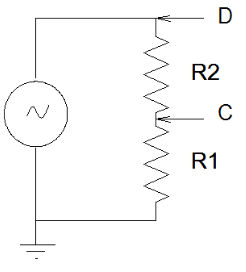
\includegraphics[width=7.5cm]{B-circ}
            \caption{Circuito Utilizado na parte B}
            \label{fig:B-circ}
        \end{figure}
    \subsection{Gráficos}
        \begin{figure} [H] 
            \begin{subfigure}[b]{7cm}  
                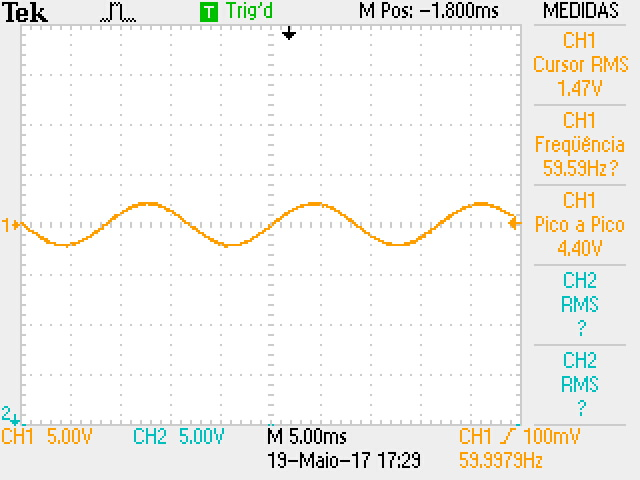
\includegraphics[width=7cm]{B-gnd-c}
                \caption{Nos pontos GND e C}
                \label{fig:B-gnd-c}
            \end{subfigure}
            \begin{subfigure}[b]{7cm}  
                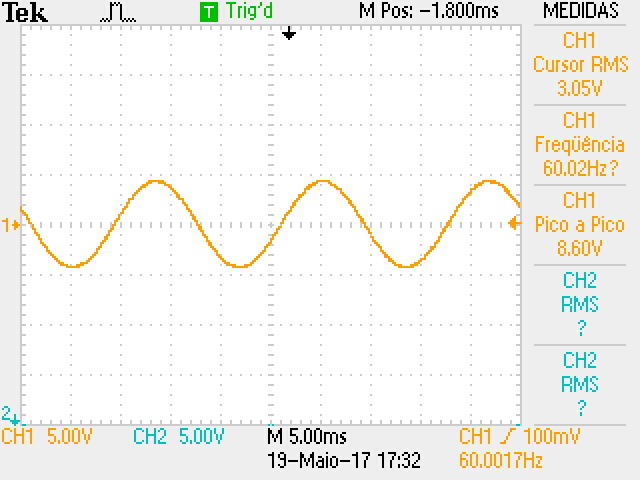
\includegraphics[width=7cm]{B-gnd-d}
                \caption{Nos pontos GND e D}
                \label{fig:B-gnd-d}
            \end{subfigure}
                \caption{Gráfic Uxt no oscilador na parte B}
        \end{figure}
    \subsection{B1}
        \paragraph{Para ponto C e usando os cursores} foi encontrado:
        $$V_p = (2,0 \pm 0,3)V$$
        $$T = (17 \pm 3)ms$$
        $$\omega = (0,37 \pm 0,02)rad/ms$$
        $$f = (60 \pm 10)Hz$$

        Sendo as incertezas encontradas a partir 
        da função de precisão do osciloscópio 
        dada pelo “Série TBS1000 Osciloscópios de 
        Armazenamento Digital ZZZ Manual do Usuário”:
        $$\pm(3\% de |leitura| + 0,1 div + 1mV)$$
        para a configuração vertical (tensão) 
        do osciloscópio.
        $$\pm(0,01\% de |leitura| + 1 div + 0,4ns)$$
        para a configuração horizontal (tempo) 
        do osciloscópio.

        Ou por propagação de erro:
        $$\omega = \frac{2\pi}{T} \Rightarrow \Delta \omega^2 = (\frac{d\omega}{dT})^2 \Delta T^2 \Rightarrow \Delta \omega = \pm\frac{2\pi}{T^2} \Delta T$$
        $$f = \frac{1}{T} \Rightarrow \Delta f^2 = (\frac{df}{dT})^2 \Delta T^2 \Rightarrow \Delta \omega = \pm\frac{1}{T^2} \Delta T$$
        \newline

        Logo:
        $$V_p = 2,2 V$$
        $$T = 17 ms$$
        $$\omega = \frac{2\pi}{T} rad/ms = \frac{2\pi}{17} rad/ms \approx 0,37 rad/ms$$
        $$f = \frac{1}{T} Hz = \frac{1}{17*10^{-3}} Hz \approx 60 Hz$$
        \newline  
        $$\Delta V_p = \frac{(3\% de |leitura| + 0,1 div + 0,001)}{\sqrt{3}} V = \frac{(0,03*2 + 0,1*5 + 0,001)}{\sqrt{3}} V \approx 0,3 V$$
        $$\Delta T = \frac{(0,01\% de |leitura| + 1 div + 0,0000004)}{\sqrt{3}} ms = \frac{(0,01*0,01*17+5+0,0000004)}{\sqrt{3}} ms \approx 3 ms$$
        $$\Delta \omega = \Delta T\frac{2\pi}{T^2} rad/ms = 3*\frac{2\pi}{17^2} rad/ms \approx 0,06 rad/ms$$
        $$\Delta f = \Delta T\frac{1}{T^2} Hz = 3*10^{-3}\frac{1}{(17*10^{-3})^2} Hz \approx 10 Hz$$


    \subsection{B2}
        \paragraph{Utilizando a função `medida`} foi encontrado: 
        $$V_p = (2,2 \pm 0,3)V$$
        $$T = (17 \pm 3)ms$$
        $$\omega = (0,37 \pm 0,02)rad/ms$$
        $$f = (60 \pm 10)Hz$$

        Sendo as incertezas encontradas a partir 
        da função de precisão do osciloscópio 
        dada pelo “Série TBS1000 Osciloscópios de 
        Armazenamento Digital ZZZ Manual do Usuário”:
        $$\pm(3\% de |leitura| + 0,1 div + 1mV)$$
        para a configuração vertical (tensão) 
        do osciloscópio.
        $$\pm(0,01\% de |leitura| + 1 div + 0,4ns)$$
        para a configuração horizontal (tempo) 
        do osciloscópio.

        Ou por propagação de erro:
        $$\omega = \frac{2\pi}{T} \Rightarrow \Delta \omega^2 = (\frac{d\omega}{dT})^2 \Delta T^2 \Rightarrow \Delta \omega = \pm\frac{2\pi}{T^2} \Delta T$$
        $$f = \frac{1}{T} \Rightarrow \Delta f^2 = (\frac{df}{dT})^2 \Delta T^2 \Rightarrow \Delta \omega = \pm\frac{1}{T^2} \Delta T$$
        \newline

        Logo:
        $$V_p = 2,2 V$$
        $$T = 17 ms$$
        $$\omega = \frac{2\pi}{T} rad/ms = \frac{2\pi}{17} rad/ms \approx 0,37 rad/ms$$
        $$f = \frac{1}{T} Hz = \frac{1}{17*10^{-3}} Hz \approx 60 Hz$$
        \newline  
        $$\Delta V_p = \frac{(3\% de |leitura| + 0,1 div + 0,001)}{\sqrt{3}} V = \frac{(0,03*2,2 + 0,1*5 + 0,001)}{\sqrt{3}} V \approx 0,3 V$$
        $$\Delta T = \frac{(0,01\% de |leitura| + 1 div + 0,0000004)}{\sqrt{3}} ms = \frac{(0,01*0,01*17+5+0,0000004)}{\sqrt{3}} ms \approx 3 ms$$
        $$\Delta \omega = \Delta T\frac{2\pi}{T^2} rad/ms = 3*\frac{2\pi}{17^2} rad/ms \approx 0,06 rad/ms$$
        $$\Delta f = \Delta T\frac{1}{T^2} Hz = 3*10^{-3}\frac{1}{(17*10^{-3})^2} Hz \approx 10 Hz$$

    \subsection{B3}
        \paragraph{A tensão eficaz $V_{ef}$} calculada foi:
        $$V_{ef} = (1,6 \pm 0,3) V$$
        que foi calculada como:
        $$V_{ef} = \frac{V_p}{\sqrt{2}}$$
        $$\Delta V_{ef} = \frac{1}{\sqrt{2}} \Delta V_p$$

        Logo:
        $$V_{ef} = \frac{V_p}{\sqrt{2}} V = \frac{2,2}{\sqrt{2}} V \approx 1,9 V$$
        $$\Delta V_{ef} = \frac{1}{\sqrt{2}} \Delta V_p V = \frac{0,3}{\sqrt{2}} V \approx 0,3 V$$

        Enquanto a tensão eficaz medida pelo multímetro foi:
        $$V_{ef} = 1,47 V$$

        O que está de acordo do $V_{ef}$ calculado

